% THIS IS SIGPROC-SP.TEX - VERSION 3.1
% WORKS WITH V3.2SP OF ACM_PROC_ARTICLE-SP.CLS
% APRIL 2009
\documentclass{acm_proc_article-sp}

\usepackage{graphicx}
\usepackage{epsfig}
%% The amssymb package provides various useful mathematical symbols
\usepackage{amssymb}
\usepackage{amsmath}

\begin{document}

\title{ Analyze tweets during U.S Presidential debate to predict the political stance of Users
Format}

\numberofauthors{2}

\author{
% You can go ahead and credit any number of authors here,
% e.g. one 'row of three' or two rows (consisting of one row of three
% and a second row of one, two or three).
%
% The command \alignauthor (no curly braces needed) should
% precede each author name, affiliation/snail-mail address and
% e-mail address. Additionally, tag each line of
% affiliation/address with \affaddr, and tag the
% e-mail address with \email.
%
% 1st. author
\alignauthor
Abhishek K Srivastava \\
       \affaddr{University of California,Riverside}\\
       \affaddr{900 University Ave,}\\
       \affaddr{Riverside, CA, 92521}\\
       \email{asriv003@ucr.edu}\\
% 2nd. author
\alignauthor
Ravdeep S Pasricha \\
       \affaddr{University of California,Riverside}\\
       \affaddr{900 University Ave,}\\
       \affaddr{Riverside, CA, 92521}\\
       \email{rpasr001@ucr.edu}\\
}
\maketitle
\begin{abstract}
Twitter is a micro-blogging website where users post and read 140 character messages called ``tweets''.It is one of the most popular way of expressing ones opinion, to contribute to a trend/meme, or to react conversationally. That is why Twitter has been an interesting platform for researchers to do opinion mining.

In our project we have collected tweets during presidential debate. Using sentiment analysis we identified sentiments related to the tweets. Then we classify the tweets with sentiment value to the candidates. Our evaluation shows that micro-blogging websites like twitter can be used to find general opinion of users regarding their political stance.

\end{abstract}

\section{Introduction}
Social media has a massive influence on our current society and culture. It has become one of the most popular ways of communication among our social circle. Social media websites like Twitter, Facebook are used by businesses to advertise  their products to the mass audiences and also its been used as a forum to provide customer service,feedback and resolve customer issues.\cite{jenny:wihsmthos} The major news outlets is also using social media as a news platform and more and more people are using social media as a news source. People have
begun to use Twitter to discuss live events, which they are attending or watching on broadcast TV.

This same trends of social media marketing is being used by political parties and politicians to reach out to mass audiences to convey their policies and political agendas. In the past social media has played a crucial role in election campaigns. In 2012 U.S presidential election social media was one of the major part of Barack Obama's election campaign.

In our project we look at twitter, a micro-blogging website where millions of users share their personal thoughts on different subjects like sports, politics, movies etc. About 500 million of tweets are tweeted by users on daily basis world wide. So it has enormous amount of data which can be collected and used for opinion mining, it has been an interesting platform for researchers to find new techniques for opinion mining.

In this project we analyze the tweets of users on twitter, tweeted during U.S presidential debate to determine the political stance of the users. Our approach used for this problem was to understand the sentiments of the tweets and then classify that tweet to a particular candidate.

We built a classifier which analyze the sentiment of a tweet. After analyzing the sentiment of a given tweet, it can be classified as:
\begin{itemize}
\item Positive sentiment.
\item Negative sentiment.
\end{itemize}

Then we use this sentiment classified tweet to classify against candidates, in our case between Hillary Clinton and Donald Trump.

Presidential debates can be a ``game changers'' is a belief almost universally held by political pundits and strategists because many voters do pay attention to the debates and debate can be used as a platform to reach out to the undecided voters by conveying their policies and future plan toward country.\cite{aaSides:dpdrm}

That is why objective of our project was to determine the influence of the tweets tweeted during debates and use them a people opinion regarding the candidate and predict popular opinion. 

\section{Related Work}
Since twitter is huge source of the people's opinion and easy accessible. It has been a very popular source to gather data and is  being used it for research in the field of sentiment analysis and opinion mining.\cite{wang:asfrttsa, shamma:ttducaous}

In \textbf{Sentiment Analysis of Twitter Data }(LSM 2011) Agarwal et al \cite{aAgarwal:saotd} paper deals with detecting and analyzing an overall sentiment of tweets. Authors used following models for two classification tasks. One classifies into positive \&
negative and another into positive, negative and neutral. Models used in their paper are unigram(used as a baseline), features based and tree kernel based model. Apart from these three it also uses combinations of models: combining unigram with features based and combining features based with tree kernel. This paper demonstrated that feature based and tree kernel based model outperforms unigram model. This paper only deals with classifying tweet sentiments does not classify tweets to topic. For example given a tweet is positive whether it`s for Hillary or Trump. This can be extended to classification based on topics as well.

In \textbf{Predicting Elections with Twitter: What 140 Characters Reveal about Political Sentiment }(ICWSM 2010) Tumasjan et al \cite{bTumasjan:pewt} paper treats twitter as a forum for political discussion and whether what people tweets correlate to their opinion offline. They used LIWC software for text analysis. The aim of this paper was to answer the following questions: Whether twitter is used as forum for political discussion, whether tweets of people reflect with offline political sentiment and whether tweets can be used to predict popularity of a political party in real world. This paper concludes the social media platform like twitter can be used to understand people's political views. To use LIWC, tweets were translated from German to English. Some of the sentiment might have been lost in translation. This study did not use the sentiments provided by emoticons and acronyms. Dataset did not include tweets based on hashtags.

In \textbf{Text Categorization with Support Vector Machines: Learning with Many Relevant Features }(ECML-KDD 1998) Joachims et al \cite{cJoachims:tcwsvm} paper explains why SVM is a better classification tool than other conventional methods used for text categorization. It gives empirical and theoretical explanations for why SVM achieves substantial improvement, is robust and eliminates the need for manual parameter tuning. This paper shows that SVM consistently performs well in categorization and it can handle high dimensional data with ease and eliminates the need of feature selection, also SVM does not require parameter tuning. But the  training time of polynomial and RBF SVM can be substantial for very large data. This work can be extended by using string kernels in SVM.

In \textbf{Twitter as Corpus for Sentimental Analysis and Opinion Mining}
\cite{dPak:tacfsaaom}paper authors explained why they have chosen twitter to do sentimental analysis. They have done the analysis by collecting data and dividing it into 3 different categories: positive, negative and objective emotions. Perform linguistic analysis and train the sentimental classification system and conducted experiments and evaluated against testing data to prove the techniques works better. Author concluded that training time and classification time was very less if done with SVM or decision tree, but can be easily overfitted if proper feature selection in not done properly. The future extension was to do sentimental analysis without use of emoticons.

In this project, we analyze the sentiment of a tweet using 5 classifiers namely,
\begin{itemize}
\item Naive Bayes
\item LinearSVC
\item Multinomial Naive Bayes
\item Bernoulli Naive Bayes
\item Logistic Regression
\end{itemize}
Based on the aggregate result of these classifier we classify each tweet as positive and negative with confidence value. For example if a tweet is classified as positive by 4 classifier and negative by 1, we classify it as positive with confidence value 0.8. After sentiment analysis of all the tweets, we use our candidate classifier to determine whether tweet is for Hillary or Trump.

\begin{figure}
\centering
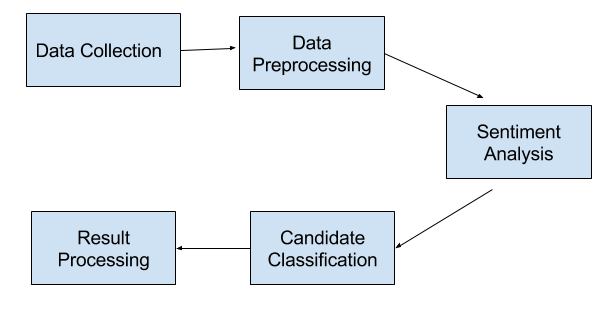
\epsfig{file=process1.png, height=2in, width=3in}
\caption{Block diagram of techniques used.}
\end{figure}

\section{Implementation}
To implement this project, we used five techniques as given below:
\begin{itemize}
\item Data Collection
\item Data Preprocessing
\item Sentiment Analysis
\item Candidate Classification
\item Result Processing  
\end{itemize}
Figure 1. Shows the flow of the whole process.
\subsection{Data Collection}
To understand the political stance of the people we collected tweets during 2nd and 3rd U.S Presidential debate. The debate running time is usually one and half hour but for better information collection we increased the window size to 5 hours. One hour before the debate starts and two and half hours after the debate is finished. 

We collected the data using Twitter's streaming API. Since we implemented our project in python, we used ``tweepy'' which is a python library for accessing the twitter API. We gather the data by passing certain keywords and hashtags(\#) like `presidentialdebate', `hillary2016', `trump', `hillary', `trump2016', `clinton', `realDonaldTrump', `HillaryClinton', `DebateNight', `debate', `elections2016' etc as a parameter to twitter streaming API. However twitter streaming API doesnot return all the tweets at a particular time. It has been estimated that using Twitter streaming API users can expect to receive anywhere from 1\% of the tweets to over 40\% of tweets in near real-time.\cite{bplanet:tfvta} The raw tweets collected was in JSON format. We collected around 1.5 million tweets during 2nd and 3rd U.S. Presidential debate.


\subsection{Data Preprocessing}
For a single tweet it has a lot of attributes which can be classified into these categories:
\begin{itemize}
	\item Twitter Info
	\item Source
	\item User Info
	\item Co-ordinates
	\item Entities etc. 
\end{itemize}
 After the data collection process we identified that for a single tweet there were many fields were empty or not necessary for our project purposes like possibly\_sensitive, filter\_level etc. After identifying such fields we parsed our data and removed those fields, which reduced the size of the data by 90\%. The cleaned data has only relevant attributes or features required for our project like user\_screen\_name, tweet\_text etc. Figure 2. shows the complete list of the attributes.

\begin{figure}
\centering
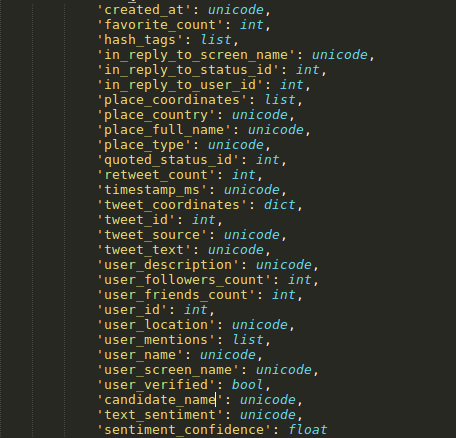
\epsfig{file=parsed.png, height=3in, width=3in}
\caption{A sample of parsed data.}
\end{figure}

\subsection{Sentiment Analysis}
Once we had the cleaned data, next step was to find the sentiment of the tweets whether it was a positive or a negative sentiment tweet. To do that we used natural language processing toolkit(NLTK). NLTK is a platform for building Python programs to work with human language data.\cite{nltk:nltkdoc}

To build a sentiment analysis classifier we needed positive and negative sentiment data to train our classifiers. We used  ``Bo Pang and Lillian Lee'' sentiment polarity datasets which was introduced in Pang/Lee ACL 2005.\cite{pang:spdmrd} It contains about 5331 positive and 5331 negative processed sentences of movie reviews.
To find the sentiment of a tweet we built a custom classifier which internally relies on following five classifiers
\begin{itemize}
\item Naive Bayes
\item LinearSVC
\item Multinomial Naive Bayes
\item Bernoulli Naive Bayes
\item Logistic Regression
\end{itemize}
We split the ``Bo Pang and Lillian Lee'' sentiment polarity datasets into training and testing dataset. We trained these five classifier with the training dataset and then we tested same classifiers with testing data. Figure 3 shows the accuracy of the classifiers and top 15 most frequent words used in the polarity dataset with their frequency occurrences in positive and negative dataset.

We build a custom classifier which classifies a tweet as positive or negative after getting result from all the 5 classifiers and assigns a confidence value to a tweet based on the number of classifier classified it a positive or negative. For example, if a tweet was classified as negative by three classifiers and as positive by two classifiers. Then a tweet is classified as negative with confidence value of $0.6$ calculated as $\frac{3}{5}$.

\begin{displaymath}
 \text{sentiment confidence} = \frac{\text{Number of majority classifier}}{\text{Total Number of classifiers}}
\end{displaymath}

Once our custom classifier was designed, we ran it against the complete dataset of tweets we had collected and cleaned.To store the value of sentiment and confidence we used custom attribute text\_sentiment and sentiment\_confidence.

\begin{figure}
\centering
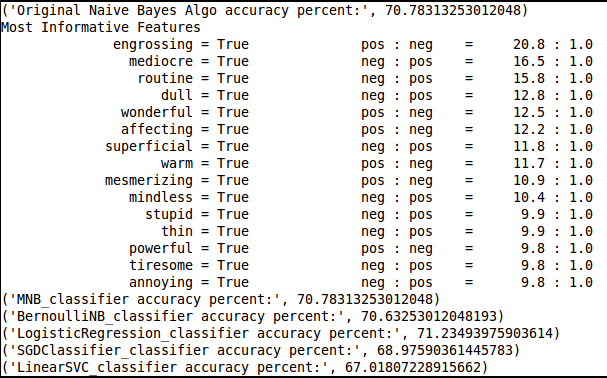
\epsfig{file=sentiment.png, height=2in, width=3in}
\caption{Accuracy of classifiers used.}
\end{figure}

\subsection{Candidate Classification}
At this stage we had classified each tweet as positive and negative sentiment with a confidence value. Now we had to classify whether a tweet (positive or negative) was for Hillary or Trump.
To achieve this we looked through each tweet text for certain keywords for each candidate. So to classify a tweet for Hillary we looked at the keywords like: 
\begin{itemize}
\item `liberal', `hillary', `clinton', `democrat', `lockherup', `progessive', `kaine', `democratic', `hillary2016'.
\end{itemize}
And for Trump we looked at keywords like:
\begin{itemize}
\item `trump', `donald', `republicans', `conservative', `maga', `lockhimup', `pence', `trump2016'
\end{itemize}
We ran this technique against 1.3 million tweets and we classified around 900,000 tweets among the 
candidates. And around 400,000 tweets were not able to classified against any candidate and were marked as neutral.

\begin{figure}
\centering
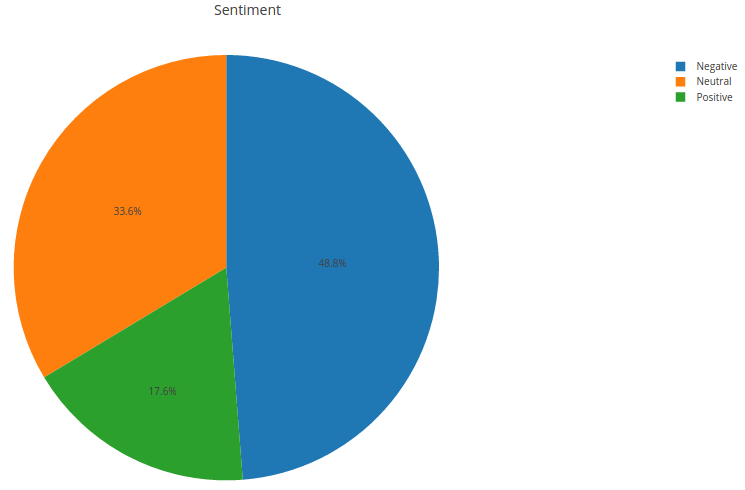
\epsfig{file=result3.png, height=1.25in, width=2in}
\caption{Overall sentiment of tweets.}
\end{figure}

\begin{figure}
\centering
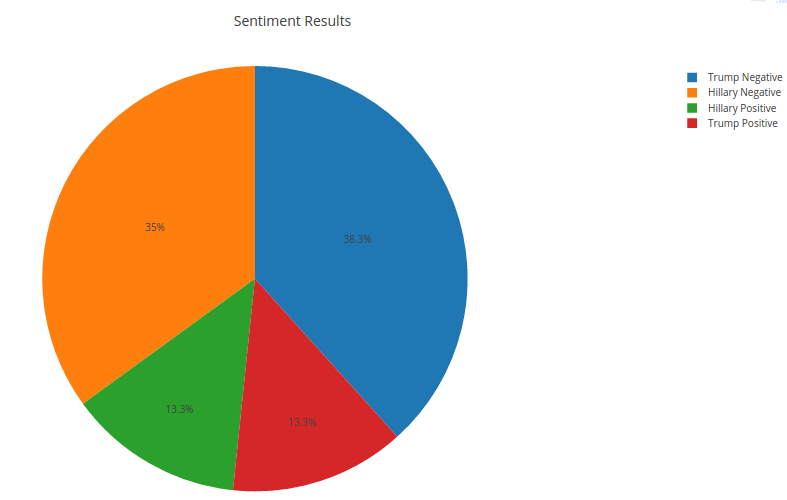
\epsfig{file=result1.png, height=1.25in, width=2in}
\caption{Sentiment related to particular candidates.}
\end{figure}

\begin{figure}
\centering
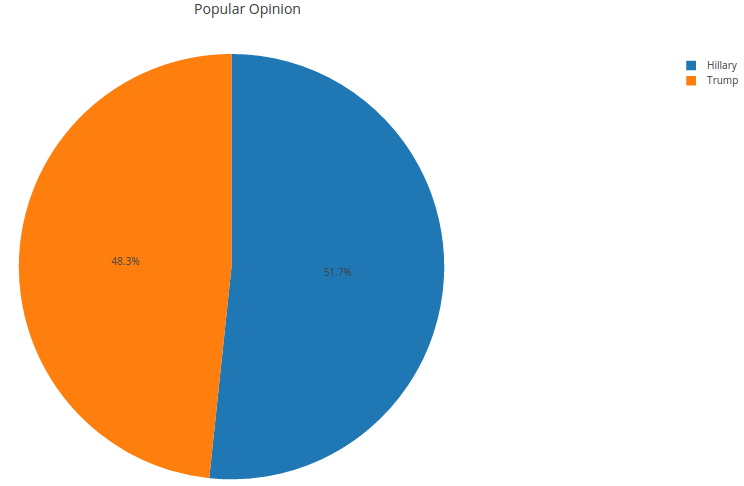
\epsfig{file=result2.png, height=1.25in, width=2in}
\caption{Final Results.}
\end{figure}

\subsection{Result Processing}
After classifying positive and negative sentiment tweets to particular candidates. We needed to visualize these insights. Since we stored our data in MongoDB, we were able to use Metabase to learn about these insights. Metabase is an opensoure analytics tool, which lets you find insights on your data.\cite{metabase:mbdb} We also used `plot.ly` to plot certain graphs. \cite{plotly:graphplot}
Using Metabase we were able to find users with high frequency of tweets. Most of those users were major news outlets like ABC, CNN, FOXnews or candidates themselves. We did removed tweets from consideration by major news outlet and candidate themselves.(Shown in result findings)  

\section{Result and Findings}
We ran our sentiment classier and candidate classification module on around 1.3 million tweets. Below are our findings:
\begin{itemize}
	\item Out of 1.3 million tweets around 893,811 were classified as either for Trump or Hillary. 
	\item Remaining tweets roughly about 400,000 were not classified to any candidate. So were marked as neutral.
	\item Out of 893,811 candidate classified tweets, 432,357 were classified as Hillary with both positive and negative sentiments
	\item And 461,454 were classified as Trump with both positive and negative sentiments.
	\item After removing tweets of major news outlets and candidates from consideration these numbers dropped to 427,504 and 456,656 for Hillary and Trump respectively.
\end{itemize}
To compute the popularity of a candidate, we add the count of positive tweets of candidate with count of negative tweets of the opponent. Here we are assuming that if a user tweets negative about a candidate, that user probably supports the other candidate but that might not be the case in reality.

\begin{figure*}
	\centering
	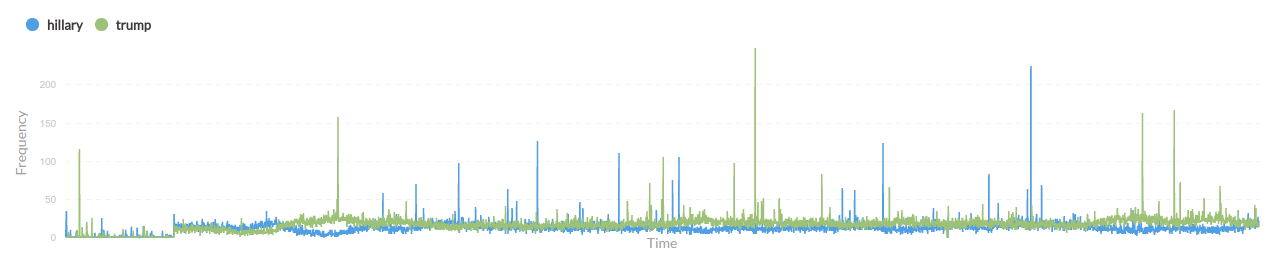
\epsfig{file=Oct09.png, height=1.5in}
	\caption{Time Series of number of tweets tweeted for the candidate on October 09 during debate.}
\end{figure*}

\begin{figure*}
	\centering
	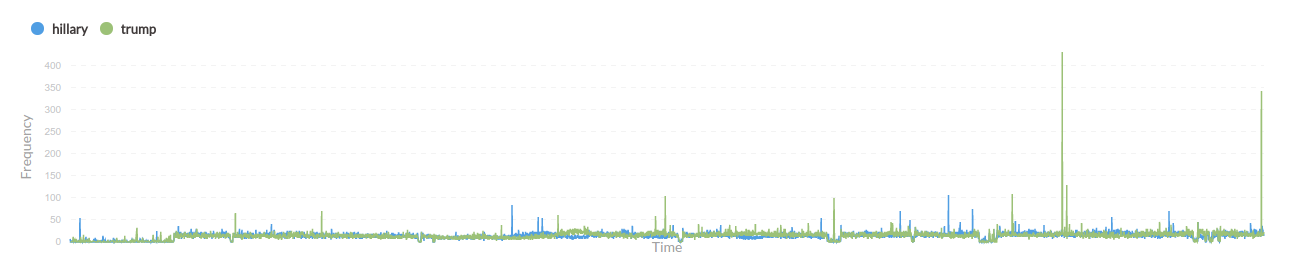
\epsfig{file=Oct19.png, , height=1.5in}
	\caption{Time Series of number of tweets tweeted for the candidate on October 19 during debate.}
\end{figure*}

\begin{figure}
	\centering
	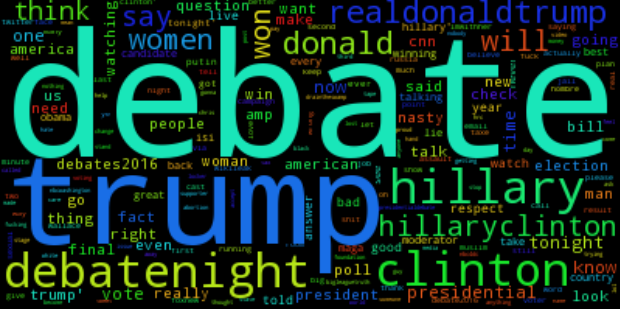
\epsfig{file=wordcloud1.png, height=1.5in, width=3in}
	\caption{Word Cloud from tweeted texts.}
\end{figure}

\begin{table}
	\centering
	\caption{Distribution of positive and negative sentiment among the candidates.}
	\begin{tabular}{|c|c|l|} \hline
		Candidate&Positive&Negative\\ \hline
		Hillary Clinton & 117986 & 309518\\ \hline
		Donald Trump & 117794 & 338862\\ \hline
	\end{tabular}
\end{table}

\begin{table}
	\centering
	\caption{Popularity of the candidates.}
	\begin{tabular}{|c|l|} \hline
		Candidate&Popularity Count\\ \hline
		Hillary Clinton & 456848\\ \hline
		Donald Trump & 427312\\ \hline
	\end{tabular}
\end{table}

\begin{itemize}
	\item So to compute the popularity for Hillary, we combine count of Hillary positive tweets with Trump negative tweet.
	\item And to compute popularity for Trump, we combine count of Trump positive tweets with Hillary negative tweet.
\end{itemize}
Table 1 shows the distribution of positive and negative tweets among the candidates.
Table 2 shows the popularity of candidates.

We use data mentioned in tables to plot few pie charts
\begin{itemize}
	\item Figure 4 shows the the percentage distribution of sentiment of tweets.
	\item Figure 5 shows the percentage distribution of sentiment of tweets for both candidates
	\item Figure 6 shows the percentage distribution of the popularity of candidates based on Table 2
	\item Since we collected data real time during dedates, we were able to plot the time-series of the data collected. Which shows the number of tweets tweeted for each candidate. This is shown in Figure 7 and 8.
	\item Figure 9 shows the word cloud of the most frequent words used in our dataset.
\end{itemize}

\section{Conclusions}
After completing all the steps mentioned above we reached to the conclusion that from the tweets we collected during the 2nd and 3rd U.S Presidential debate shows Hillary Clinton as a popular opinion among the users. We can also conclude that there is more negative sentiments towards both of the candidate than positive sentiments.  
%\end{document}  % This is where a 'short' article might terminate

\section{Future Work}
There is a lot of work can be done to improve this project. Few of them are listed below:
\begin{itemize}
	\item Sentiment Analysis : We are using training data for our sentiment classifier as a movie review samples attached with positive and negative sentiment so we can improve the accuracy of the twitter sentiments by creating our own training sample from twitter data for both positive and negative sentiments.
	\item Candidate Classification : We are doing candidate classification based on the keywords attached to the candidates in the twitter text which can further improved.
	\item Sarcasm Detection : A lot of tweets are just plane jokes and have nothing to do with their political stance but classifying them and ignoring them from among millions of tweets is very hard task and doing so will definitely improve the accuracy of the classifiers.
\end{itemize}

%ACKNOWLEDGMENTS are optional
\section{Acknowledgments}
We would like to thank Professor Vagelis Papalexakis for his advice throughout the project and his guidance. Also we would like to thank Twitter to let us mine their data and multiple other resources which help us learn new things and helped us finish our project.\cite{ppdn:pythonprog, sklearn:skikit, tapi:twitterapi, wiki:wikipedia}

%
% The following two commands are all you need in the
% initial runs of your .tex file to
% produce the bibliography for the citations in your paper.
\bibliographystyle{abbrv}
\bibliography{sigproc}  % sigproc.bib is the name of the Bibliography in this case
% You must have a proper ".bib" file
%  and remember to run:
% latex bibtex latex latex
% to resolve all references
%
% ACM needs 'a single self-contained file'!
%
%APPENDICES are optional
%\balancecolumns
\appendix
%Appendix A
\section{Abstarct}
\subsection{Introduction}
\subsection{Related Work}
\subsection{Implementation}
\subsubsection{Data Collection}
\subsubsection{Data Processing}
\subsubsection{Sentiment Analysis}
\subsubsection{Candidate Classification}
\subsubsection{Result Processing}
\subsection{Result and Findings}
\subsection{Conclusions}
\subsection{Future Works}
\subsection{Acknowledgments}
\subsection{References}

% That's all folks!
\end{document}